

\chapter{绪论}

%本模板根据浙江大学研究生院编写的《浙江大学研究生学位论文编写规则》~\cite{zjugradthesisrules},
%在原有的 zjuthesis 模板~\cite{zjuthesis}基础上开发而来。

%本模板的本科生版本\cite{zjuthesisrules}得到了浙江大学本科生院老师的支持与审核,
%已经在本科生院网上公示。
%但当前的研究生版本并未经过研究生院老师的审核,
%同学们使用时要注意对照模板与要求,
%切不可盲目使用。

%作者本人并未编写过浙江大学研究生毕业论文,
%所以不清楚具体要求。
%如果有热心同学愿意帮忙,
%可以替我联系相关老师,我会配合审核并修改代码。

\section{背景}

% 如果你在Overleaf上编译本模板,请注意如下事项:

% \begin{itemize}
%     \item 删除根目录的 ``.latexmkrc'' 文件,否则编译失败且不报任何错误
%     \item 字体有版权所以本模板不能附带字体,请务必手动上传字体文件,并在各个专业模板下手动指定字体。
%         具体方法参照 GitHub 主页的说明。
%     \item 当前的Overleaf默认使用TexLive 2017进行编译,但一些伪粗体复制乱码的问题需要TexLive 2019版本来解决。
%         所以各位同学可以在Overleaf上编写论文时务必切换到TexLive 2019或更新版本来编译,以免产生查重相关问题。
%         具体说明参照 GitHub 主页。
% \end{itemize}


\section{研究现状}

% 我们可以用includegraphics来插入现有的jpg等格式的图片,
% 如\autoref{fig:zju-logo}所示。

\begin{figure}[htbp]
    \centering
    \includegraphics[width=.3\linewidth]{logo/zju}
    \caption{\label{fig:zju-logo}浙江大学LOGO}
\end{figure}

重点突出目前的研究处于什么状态,尚存在的问题

\subsection{体数据相关性分析}
\subsection{体数据特征提取}
\subsection{体数据表征学习}
\section{本文工作及组织结构}


\par 如\autoref{tab:sample}所示,这是一张自动调节列宽的表格。

\begin{table}[htbp]
    \caption{\label{tab:sample}自动调节列宽的表格}
    \begin{tabularx}{\linewidth}{c|X<{\centering}}
        \hline
        第一列 & 第二列 \\ \hline
        xxx & xxx \\ \hline
        xxx & xxx \\ \hline
        xxx & xxx \\ \hline
    \end{tabularx}
\end{table}


\par 如\autoref{equ:sample},这是一个公式

\begin{equation}
    \label{equ:sample}
    A=\overbrace{(a+b+c)+\underbrace{i(d+e+f)}_{\text{虚数}}}^{\text{复数}}
\end{equation}

\chapter{体数据嵌入表征的学习与应用}

\section{传统的体数据信息表达(TODO:在后面提及,本节不写)}
\subsection{基于数值统计的信息表达方法(TODO:在第三章、第四章提及)}
通过挖掘体数据内部的属性,如标量值、梯度、统计学等信息对数据进行深层次表达

【数据压缩】

【统计分布】

\subsection{基于拓扑结构的信息表达方法(在第五章提及)}

通过树、图等数据组织方式对数据进行抽象表征(TODO:暂不提及)

【contour tree】

【Reeb Graph】

【nested tracking graphs (2017)】

【Dynamic nested tracking graphs (2019)】

【fiber surfaces: Generalizing isosurfaces to bivariate data (2015)】

【Transgraph: Hierarchical exploration of transition relationships in time-varying volumetric data (2011)】

【persistence diagram】

【Graphs in scientific visualization: A survey (2017)】

【Joint contour nets (2014)】


\section{体数据相关性分析}
\subsection{体素相关性}
\subsection{数值相关性}
\subsection{体数据整体相关性}
\subsection{特征相关性}

【Transgraph: Hierarchical exploration of transition relationships in time-varying volumetric data (2011)】

\section{体数据特征提取}
\subsection{单变量体数据特征提取}

基于传统方式的特征提取方法

【Texture-based transfer functions for direct volume rendering (2008)】

【State of the art in transfer functions for direct volume rendering (2016)】

基于机器学习的特征提取方法

【Semi-automatic generation of transfer functions for direct volume rendering (1998)】

【An intelligent system approach to higher-dimensional classification of volume data (2005)】

【Featurelego: Volume exploration using exhaustive clustering of super-voxels (2019)】

【An Intelligent System Approach for Probabilistic Volume Rendering using Hierarchical 3D Convolutional Sparse Coding (2019)】

【Learning probabilistic transfer functions: A comparative study of classifiers (2018)】

\subsection{多变量体数据特征提取}
【Biclusters based visual exploration of multivariate scientific data visualization (2018)】

【Easyxplorer: A flexible visual exploration approach for multivariate spatial data (2015)】

【Guideme: Slice-guided semiautomatic multivariate exploration of volumes (2014)】

\subsection{时序体数据特征提取}
特征演化

【nested tracking graphs ((2017))】

【Dynamic nested tracking graphs (2019)】

特征追踪

【】


\section{基于深度学习的体数据分析方法/深度学习在体数据中的应用}
传统的体数据表达缺陷

深度学习方法

特征-based

【Flownet: A deep learning framework for clustering and selection of streamlines and stream surfaces (2018)】

【Insitunet: Deep image synthesis for parameter space exploration of ensemble simulations (2020)】

体数据-based

【A deep learning approach to selecting representative time steps for time-varying multivariate data (2019)】

【V2v: A deep learning approach to variable-to-variable selection and translation for multivariate time-varying data (2020)】

【Tsr-tvd: Temporal super-resolution for time-varying data analysis and visualization (2020)】

体素-based

【An intelligent system approach to higher-dimensional classification of volume data】

【A Cluster-Space Visual Interface for Arbitrary Dimensional Classification of Volume Data】


\subsection{基于图论的体数据表征学习}

树、图的进一步表征()

【】


\chapter{一种基于自然语言处理的体数据嵌入表征学习方法}

\section{引言}

为了描述复杂的物理现象,科学模拟(例如计算流体力学模拟和气象模拟)通常会产生大规模的时变和多变量的科学体数据。模拟过程中还可以设置不同参数数值,通过组集数据模拟不同条件下的现象~\cite{BURCKNER:2010:RDE}。例如,在小行星撞击海平面的模拟过程中,可通过参数控制小行星以不同的半径、速度、角度入射到空气、海平面、海水中,且随着时间的推移,行星的速度、场内的温度、周围的压强等不同变量的也具有不同的演化特性及关联规律。因此,有必要对体数据中的特征进行分类,并探索体数据之间的关联,以帮助领域专家有效地理解这些复杂的现象。

与单变量体数据的特征不同,多变量体数据的特征通常是由不同空间区域内多个变量的不同标量值组合定义的~\cite{GUO:2012:SMV}~\cite{LIU:2015:AAF}~\cite{LU:2017:MVD}。这些特征往往具有变量依赖及空间依赖。因此,对于一个复杂的物理现象,仅分析单个变量很难甚至不可能提取出重要的特征。近年来,许多工作提出了基于多元传递函数的交互式特征提取方法,通过挖掘标量值组合的方式提取特征,例如平行坐标~\cite{Inselberg:1985:TPW}~\cite{GUO:2011:MTF}~\cite{GUO:2012:SMV}和散点图矩阵~\cite{LIU:2015:AAF}。这些交互式方法的可扩展性较高,然而,对于没有先验知识的用户而言,提取有意义的特征仍然是一个繁琐且具有挑战性的过程。这是因为标量值组合的可探索空间较大,且具有大量的冗余信息。正如Parsons等人所述,大多数重要的特征通常只与特定的变量和标量值相关联~\cite{PAR:2004:SCF}。因此,亟待需要引入一种自动或半自动的多变量体数据特征分类方法来实现对特征的自动化或半自动化提取,降低用户与数据的交互,提高分类效率。

时变和组集体数据具有大量的下游分析任务,例如时变体数据中的关键时间步选择~\cite{ZHOU:2018:KTS}~\cite{PORTER:2019:ADL},特征追踪~\cite{WANG:2013:SPF}及特征演化~\cite{LUKASCZYK:2017:NTG}~\cite{LUKASCZYK:2019:DNT},以及组集体数据的三维空间探索~\cite{LEISTIKOW:2019:AEV}及参数空间探索~\cite{BURCKNER:2010:RDE}。以上分析任务大多依赖于体数据之间的数值关联及空间关联。数值关联主要度量体数据之间整体标量值的相关程度,常用的方法有Pearson相关系数和互信息。Pearson相关系数在假设体数据之间呈现正态分布的情况下度量其之间的线性依赖关系~\cite{SAUBER:2006:MAA}~\cite{SUKHAREV:2009:CSO},互信息则基于信息熵度量更一般(非线性)的依赖关系~\cite{BISWAS:2013:AIF}~\cite{DUTTA:2017:PIG}。空间关联主要基于空间结构估计体素~\cite{SAUBER:2006:MAA}~\cite{NAGARAJ:2011:AGC}之间的关联,或者估计拓扑结构~\cite{SCHNEIDER:2008:ICO}~\cite{SCHNEIDER:2013:ICO}~\cite{CARR:2014:JCN}之间的关联。数值关联及空间关联是体数据内重要的结构特征,两者之间也具有紧密的联系,例如飓风眼中心的温度与湿度紧密相关,而飓风眼外围的风速和压强关联程度较高。然而,已有的研究工作独立并没有考虑两者之间的关联,往往侧重一个层面。为此,本章将每个标量值的上下文分布编码为低维向量,将两种关联结合起来,探讨同不同体数据之间标量值的关联性。

基于等值面的相似性度量方法(ISM)~\cite{BRUCKNER:2010:ISM}使用等值面作为每个标量值的中间表征,并采用等值面的空间邻近性来度量两个标量值之间的相似性。受此启发,本章提出了一种基于标量值空间邻近度的无监督表示学习模型,为每个标量值生成一个低维向量作为其嵌入表征。在此,每个体素的标量值被看作为符号,例如自然语言中的一个单词。在多变量体数据中,该符号被解释为标量值组合。体数据中,每个体素都具有一个或多个标量值,每个体素的标量值/标量值组合上下文定义为该体素相邻体素的标量值/标量值组合。在表征学习中~\cite{BENGIO:2013:RLA},如果两个符号有相似的上下文,则它们在语义上是相似的,例如自然语言中的同义词。在体数据中,如果两个标量值/标量值组合具有相似的上下文,它们通常具有高度的相似性,属于同一特征。类似于word embedding~\cite{COLLOBERT:2011:NLP} ,本章采用基于负采样的Skip-Gram~\cite{MIKOLOV:2013:EEO}~\cite{MIKOLOV:2013:DRO}模型学习每个标量值的嵌入表征。标量值之间的相似性可以通过余弦距离直接量化。word embedding中采用了基于频率的负采样方法来提高训练效率~\cite{MIKOLOV:2013:EEO}。在体数据中,标量值的数量通常远低于自然语言中单词的数量,一些正样本可能被看作成负样本采样。因此,本章也改进了负采样策略,保证voxel2vec能够学习到标量值中更加丰富潜在信息。

本章提出了一种新的无监督式学习模型voxel2vec,通过标量值上下文分布关系学习标量值的嵌入表征。这些嵌入表征被可以用来量化标量值之间的相似性。对于单变量数据而言,一个标量值的空间分布是其等值面,标量值之间的空间邻近性等价于等值面的相似性。因此,voxel2vec可以生成类似于ISM的相似性度量结果。对于多变量数据,本章扩展了voxel2vec来量化标量值组合的相似性,并将其应用于特征分类,以验证该模型的有效性和实用性。对于时变和集合数据,本章提出了基于学习voxel2vec模型的迁移预测来分析体数据之间的关联。

本章节的贡献如下:
\begin{itemize}
\item 一个无监督的表征学习模型,自动学习上下文分布的体数据标量值/标量值组合的嵌入表征;
\item 基于多变量体数据标量值组合嵌入表征的特征分类任务;
\item 基于时变和组集体数据迁移预测的关联分析任务。
\end{itemize}

\begin{figure}[htbp]
	\centering
	% Requires \usepackage{graphicx}
	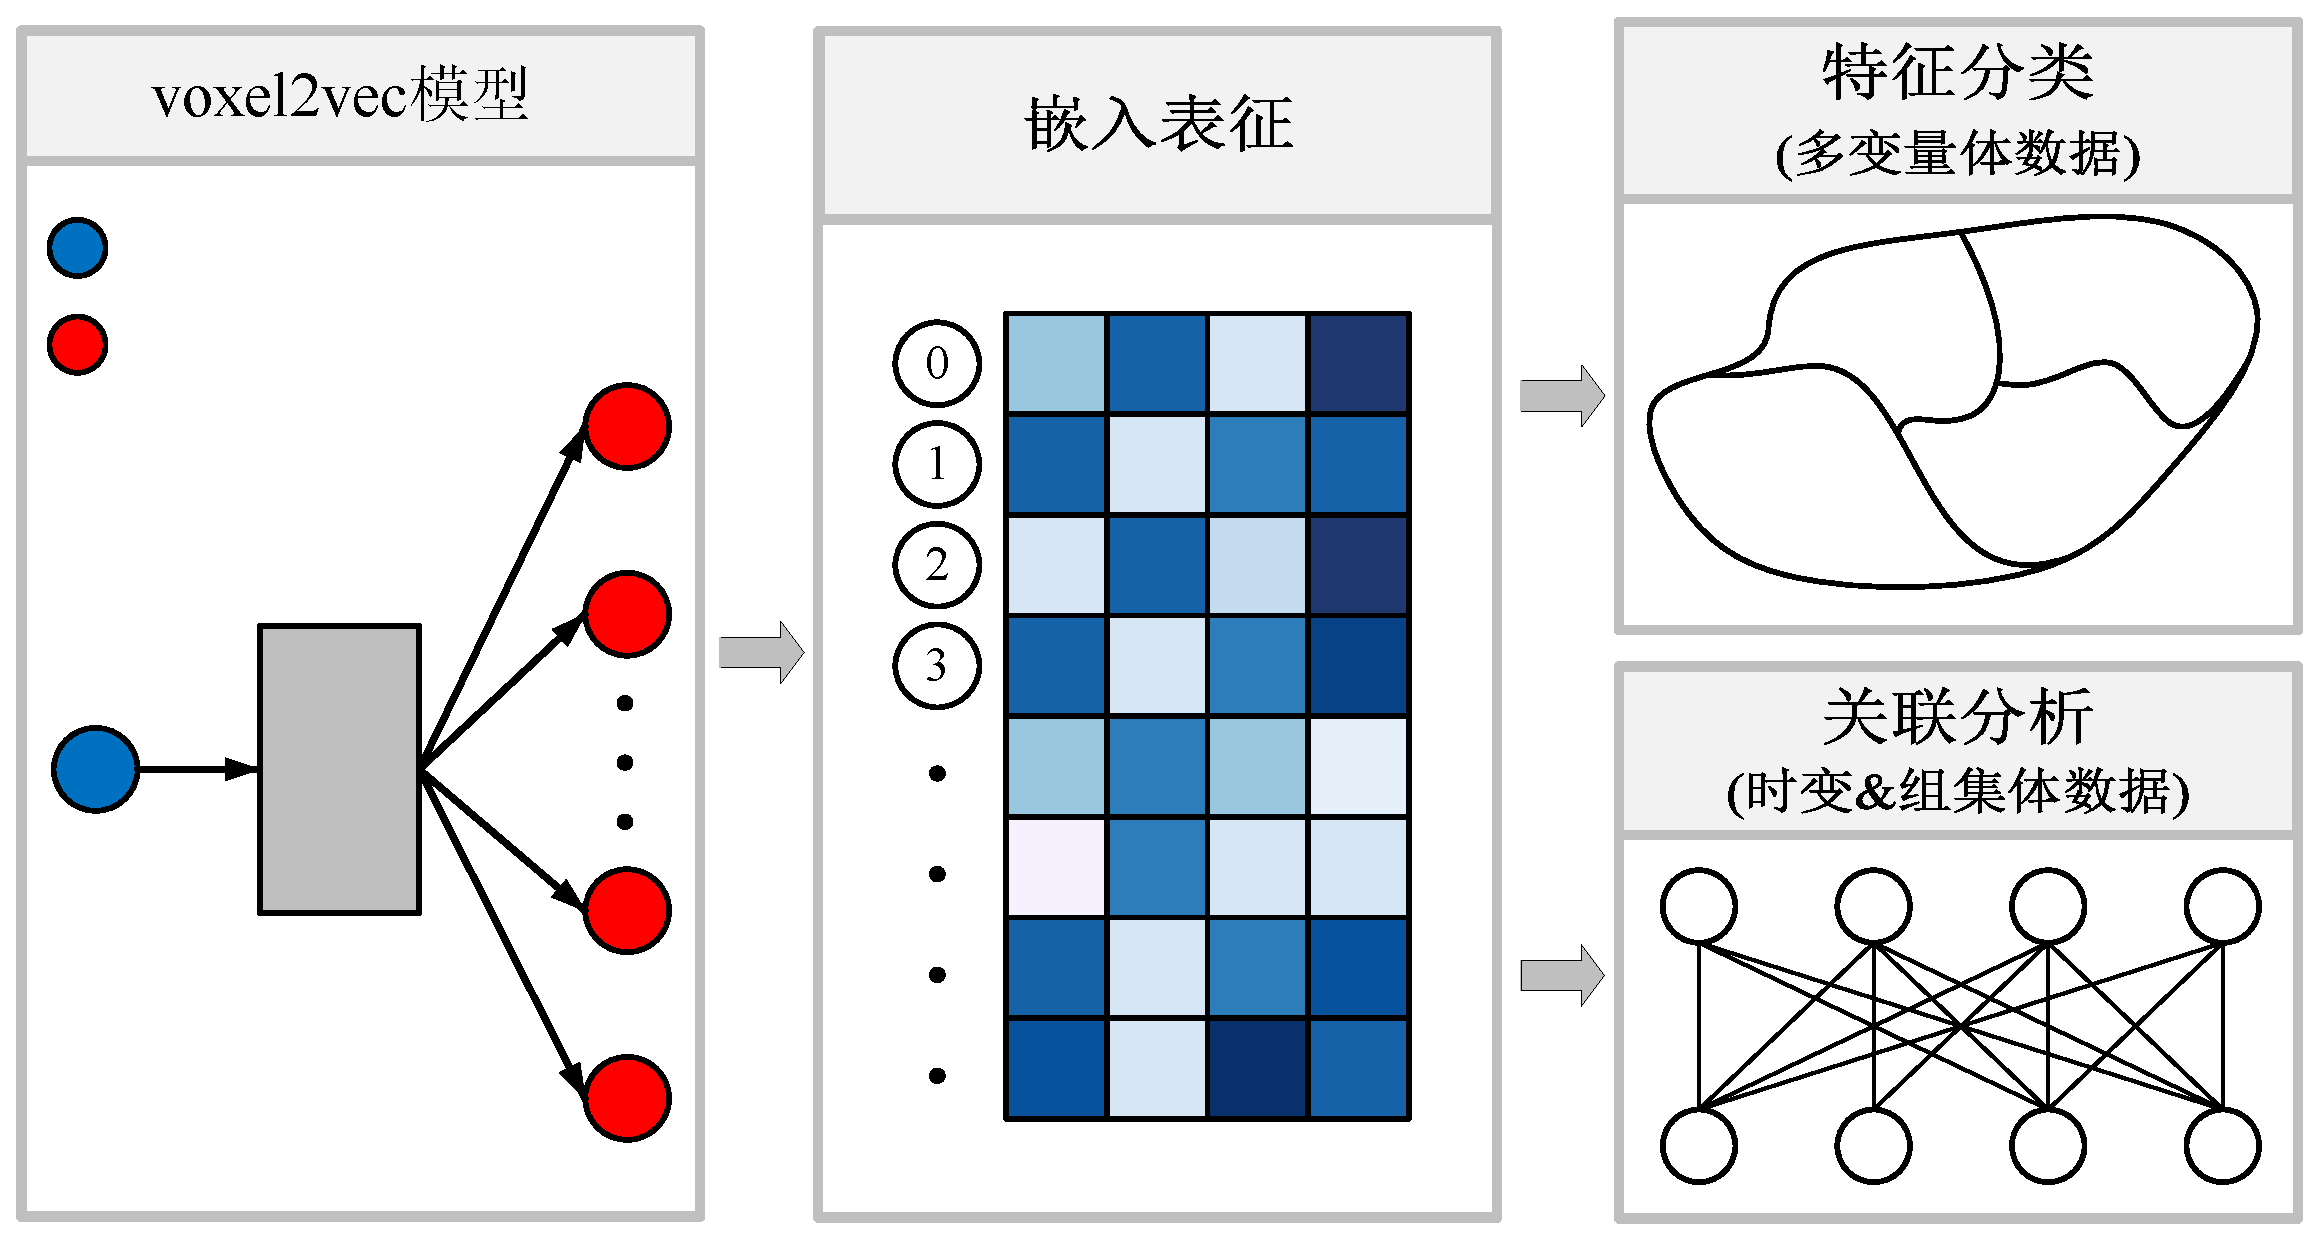
\includegraphics[width=0.7\linewidth]{voxel2vec/voxel2vec_framework.eps}
	\caption{
        voxel2vec的基础架构及标量值/标量值组合嵌入表征的下游任务。
	}\label{fig:basic_framework}
\end{figure}

\section{voxel2vec}

在自然语言处理中,神经语言模型可以将单词嵌入到低维向量空间中,以获取单词的句法和语义信息。具有负采样的Skip-Gram模型~\cite{MIKOLOV:2013:DRO}是一种自然语言处理中学习词嵌入的框架,已广泛应用于词类比~\cite{BOJANOWSKI:2017:EWV}、命名实体识别~\cite{ZIRIKLY:2015:NER}、文本分类~\cite{LAI:2015:RCN}和机器翻译~\cite{ZHANG:2014:BPE}等下游任务中。本小节搭建voxel2vec模型,通过Skip-Gram将体数据中的标量值/标量值组合表示为嵌入表征,以捕获它们之间的复杂关系,特别是语义相似性。该嵌入表征可用于体数据的特征分类和关联分析,如\autoref{fig:basic_framework}所示。

在表征学习过程中,一个体数据中的所有体素对应的标量值/标量值组合都被视为文本,也即一个符号,例如25。标量值的集合定义为$C$,因为许多体素具有相同的标量值,所以标量值的数量($|C|$)低于体素的数量。对于每个标量值$c \in C$,voxel2vec学习一个向量$z_c \in \mathbb{R}^d$,其中$d$是向量空间的维数。因此,每个标量值的嵌入表征是一个矢量。学习过程中,语义相似的标量值(例如,体数据中的相同特征)在嵌入空间中的距离将被不断拉进。本节首先描述了Skip-Gram模型,并介绍如何在体数据上下文中修改负采样策略以提高性能,最后叙述了模型的训练过程。

\begin{figure}[htbp]
    \centering
    % Requires \usepackage{graphicx}
    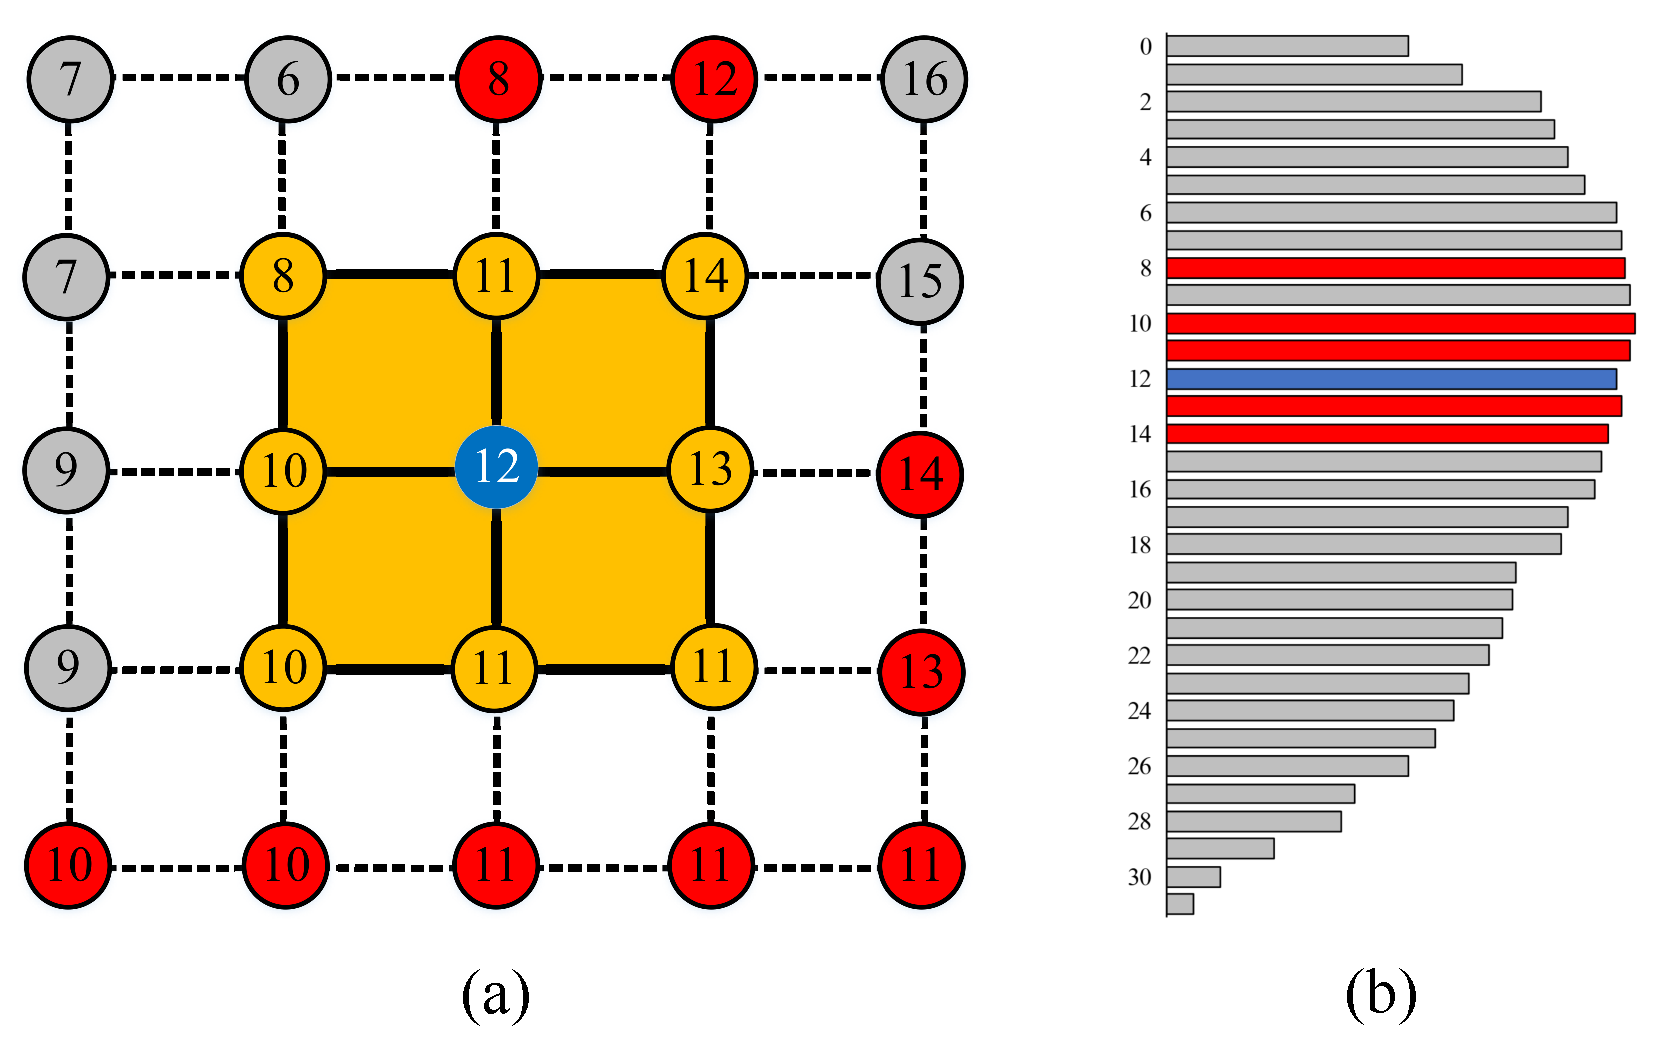
\includegraphics[width=0.7\linewidth]{voxel2vec/popular_neighbor_problem.eps}
    \caption{负采样在二维标量场上的示意图。(a)为该标量场,标量场中的蓝色体素是当前中心体素(标量值$c_t=12$),该标量值的上下文窗口的邻居体素($n=1$)对应的上下文标量值集合$o_t$为$\{8,10,11,13,14\}$。如果上下文窗口外的体素标量值在集合$c_t \cup o_t$中,则该体素被标记为红色,否则被标记为灰色。(b)为(a)标量场对应的数值分布,其中蓝色条带为$c_t$,红色条带为集合$c_t \cup o_t$。如果负样本从(b)分布中获取,则会出现流行邻居问题。
    }\label{fig:optimization_2}
  \end{figure}

\subsection{Skip-Gram模型}

自然语言处理中,Skip-Gram模型预测单词在上下文中的共现关系,使用中心词来预测其上下文单词。训练集是一个句子序列,上下文词是句子中心词的邻域单词。Skip-Gram模型的训练目标为最大化训练集中单词对的共现概率,且最小化训练集中未出现在上下文词对的共现概率。

将标量值看作单词,体数据内每个体素对应的标量值都可被看作为训练样本,其相邻体素的标量值是该标量值的上下文。本节中,定义$n$为笛卡尔坐标系下的上下文窗口维度。因此,在三维体数据中,每一个中心标量值的上下文标量值个数为$(2n+1)^3-1$。如\autoref{fig:optimization_2}(a)所示,在二维空间中,$n=1$时中心标量值(蓝色)的上下文为其周围的8个标量值(黄色)。

对于体数据中的每一个体素,定义其标量值$c \in C$的上下文标量值集合为$o$。当$c$为中心标量值时,定义其嵌入表征为$z_c \in \mathbb{R}^d$,当$c$为上下文标量值时,定义其嵌入表征为$\hat{z}_c \in \mathbb{R}^d$。Skip-Gram模型预测给定中心标量值时的上下文标量值,并最大化目标函数如下:
\begin{equation}
    J(\theta)=\frac{1}{T}\sum_{t=1}^{T}\sum_{o_i \in o_t}log P(o_i|c_t)
\end{equation}
式中,$c_t$和$o_t$分别为第$t$个体素对应的中心标量值和其上下文标量值集合,$T$为体素的数量。例如,\autoref{fig:optimization_2}(a)的一个正样本对$(c_t, o_i)$为$(12,8)$。在中心标量值为$c_t$时候,上下文标量值为$o_i$的概率可通过嵌入表征$z_{c_t}$和$\hat{z}_{o_i}$计算:
\begin{equation}\label{sec3_probability}
    log P(o_i|c_t) = log \frac{e^{\hat{z}_{o_i}^{T}z_{c_t}}}{\sum_{w \in C} e^{\hat{z}_{w}^{T}z_{c_t}}}
\end{equation}
然而,该式需要计算所有标量值对的相似度,计算代价太高,严重影响训练效率。为此,AAA等人提出了负采样策略来简化上述计算过程。该策略在保证原始正样本的选择规律不变的情况下,将负样本增加到模型的训练中。其过程为选择一个正样本对$(c_t,o_i)$和$k$个负样本对$(c_t, w)$(其中$w$为特定的非上下文分布$P$中随机抽取一个的标量值)(例如\autoref{fig:optimization_2}(a)中$(12,7)$),不断训练一个二分类逻辑回归模型。因此,\autoref{sec3_probability}可以被近似替代为下式:
\begin{equation}\label{sec3_approximate}
    log P(o_i|c_t) = \underbrace{log \sigma(\hat{z}_{o_i}^{T}z_{c_t})}_{\text{正样本}} + \underbrace{\sum_{j=1}^{k}\mathbb{E}_{w \sim P}[log \sigma(-\hat{z}_{w}^{T}z_{c_t})]}_{\text{负样本}}
\end{equation}
式中,$\sigma$为sigmoid函数,即$\sigma(x)=\frac{1}{1+e^{-x}}$。该式不断在嵌入空间中拉近在上下文中出现的标量值对,并推远未在上下文中出现的标量值对。TODO

\subsection{负采样}

负采样代替了计算所有标量值对的嵌入表征相似度,用$k$个负样本逼近目标函数,大大降低了时间复杂度,并提高了计算的精度。\autoref{sec3_probability}中定义了负样本的采样分布$P$(unigram分布~\cite{MIKOLOV:2013:DRO})。在自然语言处理中,unigram 分布刻画了单词频率的分布(比如Zipf分布),该分布假设了高频的词汇包含了更多的信息,在训练中往往具有更高的影响力。但是在在体数据,高频的标量值往往不一定包含更多的信息。例如,背景对应的标量值虽然具有大量的体素,却含有的信息量很少,不应该在训练期间频繁采样。此外,采用该分布的负采样策略还涉及到流行邻居问题~\cite{ARMANDPOUR:2019:RNS}:与中心样本高频共发的上下文样本会被作为负样本采样的概率也较高,但其本质上应该属于正样本,而非负样本。
但是如果采用unigram分布的话,相邻体素的标量值频率高于其他标量值,因此它们更有可能被作为负样本进行采样,如\autoref{fig:optimization_2}(b)所示。综上,原生的负采样策略并不能完美适配体数据,为此,本节采用了适应性采样及自取代学习两种策略来改进voxel2vec的负采样。

\subsubsection{策略1:适应性负采样}

本节设计了适应性负采样策略来解决上述的流行邻居问题。在原生的负采样中,$P$是标量值频率的分布,对于每一个标量值,其分布全部一致。然而,上下文的标量值集合$o_t$不应该被采样为中心标量值$c_t$的负样本。因此,分布$P$需要将负采样限定在集合$C-\{c_t \cup o_t\}$中,即保证负样本无法在正样本集合$\{c_t \cup o_t\}$中采样到。由于每个体素的标量值对应的上下文是不同的,因此每个体素对应的分布$P$将被适应性调整。如\autoref{fig:optimization_2}(b)所示,红色标量值在上下文中出现过,不应被纳入负样本集合中,真正的负样本应从灰色标量值集合中采样。

为了进一步解决流行邻居问题,我们采用$L_2$范式惩罚嵌入表征~\cite{ARMANDPOUR:2019:RNS}。\autoref{sec3_approximate}调整如下:
\begin{equation}\label{sec3_loss}
    log P(o_i|c_t) = \underbrace{log \sigma(\hat{z}_{o_i}^{T}z_{c_t}) - \lambda \parallel z_{c_t} \parallel_2}_{\text{正样本}}  +  \underbrace{\sum_{j=1}^{k}\mathbb{E}_{w \sim P}[log \sigma(-\hat{z}_{w}^{T}z_{c_t})] - \frac{\lambda}{k+1} \parallel \hat{z}_{w} \parallel_2}_{\text{负样本}}
\end{equation}
式中,$\lambda$为整个目标函数确定的惩罚系数。在本节中的实验中,$\lambda$被设定为0.005。范式惩罚可以降低表征学习的自由度,降低过拟合的风险~\cite{FRIEDMAN:2001:TEO},为voxel2vec提供了一个更稳定的解决方案。

\subsubsection{策略2:自取代学习}

原生负采样策略是从预定义的静态分布$P$中选择样本,该分布在整个训练期间不发生变化。因此,原生负采样策略假设了每个标量值的信息量仅取决于训练前的数据分布信息。然而,标量值的信息量也与训练过程中的分布息息相关。在局部空间内,体数据内的固有规律导致了一些标量值被看做为负样本的概率应不尽相同,因此负采样策略的分布$P$应在不同阶段时着重学习不同的潜在规律。为一个好的模型选择训练样本一直是机器学习界的重要研究课题~\cite{BUDA:2018:ASS}。为了让自然语言模型模拟人类从简单概念向困难概念的学习过程,已有工作提出自取代学习~\cite{KUMAR:2010:SLF},通过当前样本的表现来自动选择训练样本。
为了提高节点分类和链接预测的精度,Guo和Huang~\cite{GAO:2018:SNE}将自取代学习应用于节点嵌入的负采样策略中。voxel2vec同样采用了自取代学习策略,从简单样本到困难样本进行动态自适应负采样。模型首先学习简单的样本,然后学习困难的样本,这样可以为模型找到一个更好的解决方案,并加快训练过程。

与自适应负采样相似,分布$P$不仅依赖于预定义的标量值静态分布,而且在训练过程中随标量值的当前信息量不断演化。给定标量值为$c_t$的中心体素,定义其负样本$w \in C$的信息量为$p(w|c_t)=\sigma(\hat{z}_{w}^{T}z_{c_t})$。如果$p(w|c_t)$较大,则$w$是一个困难样本,否则$w$为简单样本。本节基于上述信息量定义,优化负样本的选择,确定分布如下:
\begin{equation}
    p_{c_t,c_i} = \frac{
        e^{
            \hat{z}_{c_i}^{T}z_{c_t}
        }
    }
    {\sum_{j=1}^{k}e^{\hat{z}_{c_j}^{T}z_{c_t}}}
\end{equation}
式中,$c_i \in C$。由于$z_{c_t})$$\hat{z}_{c_i}$在迭代过程中不断更新,因此分布$p_{c_t,c_i}$也在训练中不断更新。


为了模拟由简单到困难的学习过程,本节在负采样过程中定义一个阈值函数$t(\eta )$来控制是否丢弃某些负样本。$t(\eta )$越小,困难样本被丢弃的概率就越高。因此,$t(\eta )$在训练前期应该设定为较低的数值,以重点训练简单样本,学习数据的大致规律;在训练后期应该设定为较高的数值,在已学习到的嵌入表征的基础上训练困难样本。$t(\eta )$的定义如下:
\begin{equation}
    t(\eta ) = max(\frac{4}{B^2}\eta^2+\frac{1}{B}, 1)
\end{equation}
式中,$B=10^3$,表示为batch size。本节采用AAA等人~\cite{}设定的默认参数,即$\eta $在训练初始阶段初始化为1,每个batch增加1,。当$p(w|c_t) \geqslant t(\eta )$时,采样$w$为负样本的概率$p_{c_t,w}$为0,即$w$被认为是被丢弃的困难样本。在训练过程中,通过不断增加$t(\eta)$来逐渐包含困难样本,并在训练中间节点时考虑所有的负样本。自取代学习通过从简单到困难负样本的学习方式,动态捕获并自反馈需要的负样本分布,提高模型的健壮性。


\subsection{模型训练}

所有的训练及后续的应用实验均在实现在一台16GB内存、Intel Core i7 3.40GHz CPU和NVIDIA GTX 1070 GPU配置上。在训练过程中,voxel2vec采样得到每个正样本$c_t$及上下文标量值集$o_t$,随后根据上述定义的两个策略为每个正样本对自适应动态采样$k$个负样本对。voxel2vec采用梯度上升的方法不断通过最大化\autoref{sec3_loss}更新嵌入表征$z_{c}$及上下文嵌入表征$\hat{z}_{c}$。\autoref{alg_process}总结了voxel2vec的训练过程,为了稳定训练,学习率$\alpha$设定为0.005。在voxel2vec的训练只使用一个epoch,因为体数据中具有大规模的体素数量,其训练样本已经足够。另外,正如Mikolov等人~\cite{MIKOLOV:2013:EEO}所述,使用一个epoch训练Skip-Gram模型比使用多个epoch训练得到的结果更好,并且效率更高。


\begin{algorithm}[t]
	\caption{voxel2vec}
	\begin{algorithmic}[1]
		\For {each sampled voxel in volume data}
		\State $c_t$ is the scalar value of the voxel;
		\State $o_t$ is the context positive sample set of the voxel;
		
		\For {each $o_{i}\in o_t$}
		\State $g \gets 1 - \sigma (\hat{z}_{o_i}^{T} z_{c_t})$;
		\State $d_1 \gets g\hat{z}_{o_i}^{T} - \lambda \frac{z_{c_t}}{||z_{c_t}||_2} $;
		\State $e \gets d_1\cdot \alpha$;
		\State $d_2 \gets gz_{c_t}$;
		\State $\hat{z}_{o_i} \gets \hat{z}_{o_i} + d_2\cdot \alpha$;
		\State Draw $k$ negative samples from distribution $P = p_{c_t, v}$ where $p_{c_t, v} = 0$ for $v\in \{o_t \cup c_t\}$ or $p(v|c_t)\geq t(\eta)$;
		
		%\State $v_{0} \gets n_{i}, y_{0} \gets 1$;
		\For {each negative sample $w$}
		\State $g \gets - \sigma (\hat{z}_w^{T} z_{c_t})$;
		\State $d_1 \gets g\hat{z}_w^{T} $;
		\State $e \gets e+d_1\cdot \alpha$;
		\State $d_2 \gets gz_{c_t} - \frac{\lambda}{k+1}\frac{\hat{z}_w}{||\hat{z}_w||_2}$;
		\State $\hat{z}_w \gets \hat{z}_w + d_2\cdot \alpha$;
		\State $p_{c_t,w} \gets \frac{exp(\hat{z}_w^T z_{c_t})}{\sum_{j=1}^{k}exp(\hat{z}_{w_j}^T z_{c_t})}$;
		\EndFor
		\State $z_{c_t} \gets z_{c_t}+e$;
		\EndFor
		
		\EndFor
	\end{algorithmic}
	\label{alg_process}
\end{algorithm}


\section{应用}
\subsection{多变量体数据特征分类}
\subsection{关联性分析}
\subsubsection{时变体数据关联性分析}
\subsubsection{组集体数据关联性分析}
\subsubsection{时变组集体数据关联性分析}

\section{讨论}
\subsection{超参数分析}
\subsection{效率分析}
\subsection{voxel2vec模型分析}
\subsection{单变量体数据上的验证}
\subsubsection{比较}
\subsubsection{负采样策略分析}
\subsection{与已有工作的对比}
\section{本章小结}

\chapter{数值-变量嵌入表征的学习与应用}
\section{引言}
\section{ScalarGCN}
\subsection{ScalarGraph}
\subsubsection{结构构建}
\subsubsection{节点特征构建}
\subsection{ScalarGCN搭建}
\subsection{模型训练}
\section{应用}
\subsection{单变量特征分类}
\subsection{多变量相关性分析}
\subsubsection{时变体数据关联性分析}
\subsubsection{组集体数据关联性分析}
\subsubsection{时变组集体数据关联性分析}
\subsection{结果分析}
\section{讨论}
\section{本章小结}

\chapter{基于图卷积网络的半监督体数据特征分类方法}
\section{引言}
\section{超体素图的生成}
\section{模型搭建}
\section{应用分析}
\section{讨论}
\section{本章小结}


\chapter{总结与展望}
\subsection{本文工作总结}
\subsection{未来工作展望}

\begin{figure}[htbp]
    \centering
    \includegraphics[width=.3\linewidth]{example-image-a}
    \caption{\label{fig:fig-placeholder}图片占位符}
\end{figure}
